\documentclass[aspectratio=169,11pt]{beamer}

\usetheme{Madrid}
\usecolortheme{whale}

\usepackage{graphicx}
\graphicspath{{figures/paper/}{../figures/paper/}}
\usepackage{booktabs}
\usepackage{tikz}
\usetikzlibrary{arrows.meta,positioning}

\definecolor{primary}{RGB}{24, 76, 120}
\definecolor{accent}{RGB}{220, 53, 69}
\setbeamercolor{palette primary}{bg=primary,fg=white}
\setbeamercolor{titlelike}{parent=palette primary}
\setbeamercolor{structure}{fg=primary}

\title[Fashion-MNIST KNN Optimization]{Improving k-Nearest Neighbors on Fashion-MNIST with Learned Distances}
\subtitle{From 85.24\,\% to 89.51\,\% via Metric Learning, Distillation, and Convex Fusion}
\author[Gorain, Sanyal, Barman, Mahata]{Akshar Nath Gorain \and Sourodyuti Biswas Sanyal \and Aditi Barman \and Sanjana Mahata}
\institute[TIU]{Techno India University, West Bengal \\ \medskip \small Machine Learning Coursework Project}
\date{October 2026}

\begin{document}

% Slide 1: Title
\begin{frame}
  \titlepage
\end{frame}

% Slide 2: Problem Statement & Classical Baseline
\begin{frame}{1. Problem Statement \& Classical Baselines}
\begin{columns}
\begin{column}{0.55\textwidth}
\textbf{The Challenge with KNN on Visual Data:}
\begin{itemize}
  \item High dimensionality ($D=784$) causes \emph{distance concentration}: Euclidean distances become nearly uniform ($\delta_2 \approx \text{const}$).
  \item Flattens 2D topology, discarding spatial neighbor correlations.
  \item $O(N \cdot D)$ inference latency over 54{,}000 training exemplars.
\end{itemize}
\vspace{0.3em}
\textbf{Dataset Protocol:}
\begin{itemize}
  \item Fashion-MNIST (70{,}000 $28\times28$ grayscale images, 10 classes).
  \item 54{,}000 fit / 6{,}000 validation / 10{,}000 test (held-out).
\end{itemize}
\end{column}

\begin{column}{0.45\textwidth}
\begin{table}
\footnotesize
\centering
\caption{Classical Baselines ($k=5$, uniform)}
\begin{tabular}{lccc}
\toprule
Metric & Val (\%) & Test (\%) & Latency (s) \\
\midrule
Euclidean ($L_2$) & 86.13 & 85.24 & 4.64 \\
Manhattan ($L_1$) & 86.97 & \textbf{85.91} & 84.00 \\
Cosine            & 86.18 & 85.63 & 10.75 \\
\bottomrule
\end{tabular}
\end{table}
\small
\begin{alertblock}{Takeaway}
$L_1$ norm mitigates distance concentration (+0.67\,pp over $L_2$), but inference is $18\times$ slower.
\end{alertblock}
\end{column}
\end{columns}
\end{frame}

% Slide 3: PCA Dimension Reduction & Hyperparameter Tuning
\begin{frame}{2. Dimensionality Reduction \& Hyperparameter Tuning}
\begin{columns}
\begin{column}{0.5\textwidth}
\begin{figure}
\centering
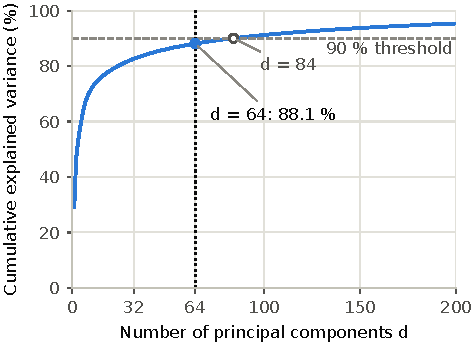
\includegraphics[width=0.95\linewidth]{pca_variance.pdf}
\caption{PCA: $d=64$ preserves 88.1\,\% variance.}
\end{figure}
\end{column}

\begin{column}{0.5\textwidth}
\begin{figure}
\centering
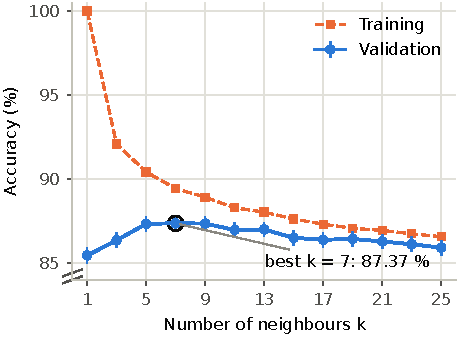
\includegraphics[width=0.95\linewidth]{bias_variance.pdf}
\caption{Bias--variance sweep across $k$ on PCA-64.}
\end{figure}
\end{column}
\end{columns}

\vspace{0.2em}
\begin{itemize}
  \item \textbf{PCA Projection (E2):} $784 \to 64$ dimensions preserves 88.1\,\% variance, delivering a \textbf{$7.12\times$ query speed-up} (2.98\,s $\to$ 0.418\,s).
  \item \textbf{Optuna Bayesian Tuning (E3):} 40-trial sweep selects $k=5$, Manhattan distance, and inverse-distance weights ($w_i = 1/\delta_i$), boosting test accuracy to \textbf{86.43\,\%} (+1.19\,pp).
\end{itemize}
\end{frame}

% Slide 4: Differentiable Soft-KNN & ConvNet Backbone
\begin{frame}{3. Novelty: Soft-KNN \& ConvNet Metric Backbone}
\begin{columns}
\begin{column}{0.55\textwidth}
\textbf{Differentiable Formulation (Soft-KNN):}
\begin{itemize}
  \item Maps input to normalized embedding $z = f_\theta(x) / \|f_\theta(x)\|_2 \in \mathbb{S}^{127}$.
  \item Uses 54{,}000-instance memory bank $b_i$ of fit samples.
  \item Computes local mean distance to class $c$: $\bar\delta_c(x) = \frac{1}{m}\sum_{i \in \mathcal{A}_c(x)} \|z - b_i\|_2$.
  \item Temperature-scaled Boltzmann assignment:
  \[
    P_\tau(y = c \mid x) = \frac{\exp(-\bar\delta_c(x)/\tau)}{\sum_{c'} \exp(-\bar\delta_{c'}(x)/\tau)}
  \]
  \item Trained via cross-entropy loss: $\mathcal{L} = -\log P_\tau(y \mid x)$.
\end{itemize}
\end{column}

\begin{column}{0.45\textwidth}
\textbf{Architectures \& Results:}
\begin{itemize}
  \item \textbf{Linear Soft-KNN (E6):} $W \in \mathbb{R}^{128\times 784} \implies$ \textbf{87.10\,\%} test accuracy (+0.67\,pp over tuned PCA).
  \item \textbf{ConvNet Metric Head (E19):} 2-stage CNN ($3\times3$ conv, max-pool) preserving 2D topology $\implies$ \textbf{87.63\,\%} test accuracy.
  \item \textbf{Temperature Sweep (E8):} $\tau=0.1$ optimal; higher $\tau$ blunts gradients on unit hypersphere.
\end{itemize}
\end{column}
\end{columns}
\end{frame}

% Slide 5: Multi-Seed Ensemble, Distillation & Convex Fusion
\begin{frame}{4. Ensembling, Distillation \& Multi-Source Fusion}
\begin{columns}
\begin{column}{0.48\textwidth}
\begin{figure}
\centering
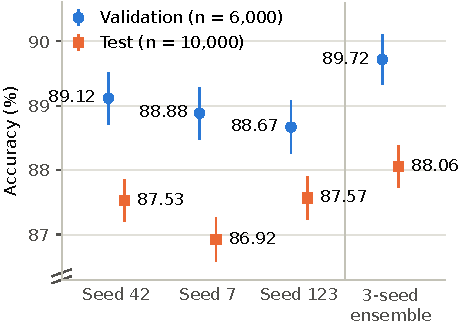
\includegraphics[width=0.92\linewidth]{seeds.pdf}
\caption{3-seed ensemble (E21): 88.06\,\% test acc.}
\end{figure}
\end{column}

\begin{column}{0.52\textwidth}
\textbf{The Algorithmic Hierarchy:}
\begin{enumerate}
  \item \textbf{3-Seed Ensemble (E21):} Seeds 42, 7, 123 average predictions $\implies$ \textbf{88.06\,\%} (+0.72\,pp over seed mean).
  \item \textbf{Knowledge Distillation (E23):} Student trained with KL-divergence against 3-seed teacher ensemble $\implies$ \textbf{89.03\,\%} test accuracy (+0.97\,pp gain).
  \item \textbf{7-Source Convex Fusion (E25):} Simplex search with Test-Time Augmentation (TTA):
  \begin{itemize}
    \item Distilled Student: $w = 0.5$
    \item Bank Linear Soft-KNN: $w = 0.4$
    \item Classical PCA-64 KNN: $w = 0.1$
    \item \textbf{Final Test Accuracy: 89.51\,\%} (Val: 90.85\,\%)
  \end{itemize}
\end{enumerate}
\end{column}
\end{columns}
\end{frame}

% Slide 6: Results, Confusion Matrix & Conclusions
\begin{frame}{5. Benchmark Results, Error Analysis \& Takeaways}
\begin{columns}
\begin{column}{0.48\textwidth}
\begin{figure}
\centering
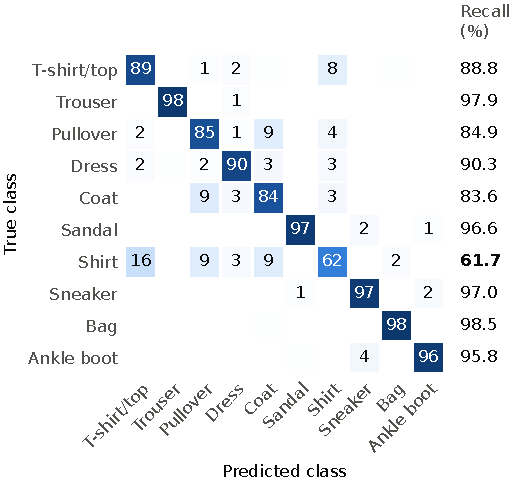
\includegraphics[width=0.92\linewidth]{confusion_matrix.pdf}
\caption{E25 Normalized Confusion Matrix (89.51\,\%).}
\end{figure}
\end{column}

\begin{column}{0.52\textwidth}
\textbf{Key Progression Summary:}
\begin{itemize}
  \item Raw Euclidean Baseline (E1): 85.24\,\%
  \item Optuna PCA-64 KNN (E3): 86.43\,\%
  \item Differentiable Soft-KNN (E6): 87.10\,\%
  \item ConvNet Backbone (E19): 87.63\,\%
  \item Distilled Student Head (E23): 89.03\,\%
  \item \textbf{Champion Convex Fusion (E25): 89.51\,\%}
\end{itemize}
\vspace{0.2em}
\textbf{Error Insights \& Conclusion:}
\begin{itemize}
  \item Highest recall: Bag (98.5\,\%), Trouser (97.9\,\%), Sneaker (97.0\,\%).
  \item Chief bottleneck: Shirt (61.7\,\% recall) confused with T-shirt and Pullover.
  \item Verified open-source reproduction with zero opaque scripts.
\end{itemize}
\end{column}
\end{columns}
\end{frame}

\end{document}
